\documentclass[11pt,a4paper, english, swedish
]{article}
\pdfoutput=1

\usepackage{custom_as}
\usepackage{multirow}

\graphicspath{ {fig_and_code/} }

%%Drar in tabell och figurtexter
\usepackage[margin=10 pt]{caption}
%%För att lägga in 'att göra'-noteringar i texten
\usepackage{todonotes} %\todo{...}

%%För att själv bestämma marginalerna. 
\usepackage[
%            top    = 3cm,
%            bottom = 3cm,
%            left   = 3cm, right  = 3cm
]{geometry}

%%För att ändra hur rubrikerna ska formateras
%\renewcommand{\thesection}{...}

\newcommand{\Thalv}[2]{\ensuremath{}T_{\nicefrac{1}{2}}\left(^{#1}\text{#2}\right)}


\begin{document}


%%%%%%%%%%%%%%%%% vvv Inbyggd titelsida vvv %%%%%%%%%%%%%%%%%

\title{K6 -- neutronaktivering av silver}
\author{Andréas Sundström}
\date{\today}

\maketitle

%\begin{abstract}
%\end{abstract}
%%%%%%%%%%%%%%%%% ^^^ Inbyggd titelsida ^^^ %%%%%%%%%%%%%%%%%

%Om man vill ha en lista med vilka todo:s som finns.
%\todolist

\section{Inledning}

\section{Metod}
Silvret först behöver först och främst neutronaktiveras, men då
behöver neutronera bromsas till rätt energier för att silverkärna
effektivt ska kunna ta upp netronerna. För att bormsa neutronerna
används framför allt väte; i den här laborationen användes parafin,
som är stora kol-vätekedjor, för att bromsa neutronerna. Alltså måste
man börja med att bestämma hur mycket parafin som behövs för att
bromsa neutronerna tillräckligt men inte heller för mycket.


\begin{figure}\centering
\resizebox{.5\textwidth}{!}{\input{fig_and_code/aktivering.pdf_t}}
\caption{}
\label{fig:aktivering}
\end{figure}


\section{Resultat och Diskussion}

\begin{table}
\centering
\caption{ }
\label{tab:diffusivitet}
\centerline{
\begin{tabular}{ll|c|c|c|}\cline{3-5}
    & & \multicolumn{1}{c|}{Rådata} & \multicolumn{1}{c|}{Bakgrundskorrigerad} & \multicolumn{1}{c|}{Rymdvinkelkorrigerad} 
    \\\hline
    % Första raden av första delen
    \multicolumn{1}{|l|}{\multirow{2}{*}{Utan kadmium}}
    &Pos. 3 & 1\,798& 1\,784& 20,5\,$\times 10^3$
    \\ \cline{2-5}
    % Andra raden av första delen
    \multicolumn{1}{|l|}{} 
    & Pos. 2 & \phantom{1\,}458& \phantom{1\,}444& \phantom{1}4,0\,$\times 10^3$
    \\\hline\hline
    % Första raden av sista delen
    \multicolumn{1}{|l|}{\multirow{3}{*}{Med kadmium}} 
    &Pos. 3 & 1\,506 & 1\,492 & 17,1\,$\times 10^3$
    \\ \cline{2-5}
    % Andra raden av sista delen
    \multicolumn{1}{|l|}{} 
    & Pos. 2 & 3\,968 & 3\,954 & 18,8\,$\times 10^3$ 
    \\ \cline{2-5}
    % Tredje raden av sista delen
    \multicolumn{1}{|l|}{} 
    & Pos. 1 & 5\,940 & 5\,926 & \phantom{1}5,9\,$\times 10^3$ 
    \\\hline
\end{tabular}}
\end{table}


\begin{figure}\centering
% GNUPLOT: LaTeX picture with Postscript
\begingroup
  \makeatletter
  \providecommand\color[2][]{%
    \GenericError{(gnuplot) \space\space\space\@spaces}{%
      Package color not loaded in conjunction with
      terminal option `colourtext'%
    }{See the gnuplot documentation for explanation.%
    }{Either use 'blacktext' in gnuplot or load the package
      color.sty in LaTeX.}%
    \renewcommand\color[2][]{}%
  }%
  \providecommand\includegraphics[2][]{%
    \GenericError{(gnuplot) \space\space\space\@spaces}{%
      Package graphicx or graphics not loaded%
    }{See the gnuplot documentation for explanation.%
    }{The gnuplot epslatex terminal needs graphicx.sty or graphics.sty.}%
    \renewcommand\includegraphics[2][]{}%
  }%
  \providecommand\rotatebox[2]{#2}%
  \@ifundefined{ifGPcolor}{%
    \newif\ifGPcolor
    \GPcolortrue
  }{}%
  \@ifundefined{ifGPblacktext}{%
    \newif\ifGPblacktext
    \GPblacktexttrue
  }{}%
  % define a \g@addto@macro without @ in the name:
  \let\gplgaddtomacro\g@addto@macro
  % define empty templates for all commands taking text:
  \gdef\gplbacktext{}%
  \gdef\gplfronttext{}%
  \makeatother
  \ifGPblacktext
    % no textcolor at all
    \def\colorrgb#1{}%
    \def\colorgray#1{}%
  \else
    % gray or color?
    \ifGPcolor
      \def\colorrgb#1{\color[rgb]{#1}}%
      \def\colorgray#1{\color[gray]{#1}}%
      \expandafter\def\csname LTw\endcsname{\color{white}}%
      \expandafter\def\csname LTb\endcsname{\color{black}}%
      \expandafter\def\csname LTa\endcsname{\color{black}}%
      \expandafter\def\csname LT0\endcsname{\color[rgb]{1,0,0}}%
      \expandafter\def\csname LT1\endcsname{\color[rgb]{0,1,0}}%
      \expandafter\def\csname LT2\endcsname{\color[rgb]{0,0,1}}%
      \expandafter\def\csname LT3\endcsname{\color[rgb]{1,0,1}}%
      \expandafter\def\csname LT4\endcsname{\color[rgb]{0,1,1}}%
      \expandafter\def\csname LT5\endcsname{\color[rgb]{1,1,0}}%
      \expandafter\def\csname LT6\endcsname{\color[rgb]{0,0,0}}%
      \expandafter\def\csname LT7\endcsname{\color[rgb]{1,0.3,0}}%
      \expandafter\def\csname LT8\endcsname{\color[rgb]{0.5,0.5,0.5}}%
    \else
      % gray
      \def\colorrgb#1{\color{black}}%
      \def\colorgray#1{\color[gray]{#1}}%
      \expandafter\def\csname LTw\endcsname{\color{white}}%
      \expandafter\def\csname LTb\endcsname{\color{black}}%
      \expandafter\def\csname LTa\endcsname{\color{black}}%
      \expandafter\def\csname LT0\endcsname{\color{black}}%
      \expandafter\def\csname LT1\endcsname{\color{black}}%
      \expandafter\def\csname LT2\endcsname{\color{black}}%
      \expandafter\def\csname LT3\endcsname{\color{black}}%
      \expandafter\def\csname LT4\endcsname{\color{black}}%
      \expandafter\def\csname LT5\endcsname{\color{black}}%
      \expandafter\def\csname LT6\endcsname{\color{black}}%
      \expandafter\def\csname LT7\endcsname{\color{black}}%
      \expandafter\def\csname LT8\endcsname{\color{black}}%
    \fi
  \fi
  \setlength{\unitlength}{0.0500bp}%
  \begin{picture}(6802.00,3968.00)%
    \gplgaddtomacro\gplbacktext{%
      \csname LTb\endcsname%
      \put(814,1326){\makebox(0,0)[r]{\strut{}$10^{2}$}}%
      \csname LTb\endcsname%
      \put(814,2514){\makebox(0,0)[r]{\strut{}$10^{3}$}}%
      \csname LTb\endcsname%
      \put(814,3703){\makebox(0,0)[r]{\strut{}$10^{4}$}}%
      \csname LTb\endcsname%
      \put(946,484){\makebox(0,0){\strut{} 0}}%
      \csname LTb\endcsname%
      \put(1674,484){\makebox(0,0){\strut{} 2}}%
      \csname LTb\endcsname%
      \put(2402,484){\makebox(0,0){\strut{} 4}}%
      \csname LTb\endcsname%
      \put(3130,484){\makebox(0,0){\strut{} 6}}%
      \csname LTb\endcsname%
      \put(3857,484){\makebox(0,0){\strut{} 8}}%
      \csname LTb\endcsname%
      \put(4585,484){\makebox(0,0){\strut{} 10}}%
      \csname LTb\endcsname%
      \put(5313,484){\makebox(0,0){\strut{} 12}}%
      \csname LTb\endcsname%
      \put(6041,484){\makebox(0,0){\strut{} 14}}%
      \put(176,2203){\rotatebox{-270}{\makebox(0,0){\strut{}$A$ /[sönderfall/min]}}}%
      \put(3675,154){\makebox(0,0){\strut{}$t$ /[min.]}}%
    }%
    \gplgaddtomacro\gplfronttext{%
      \csname LTb\endcsname%
      \put(5682,3486){\makebox(0,0)[r]{\strut{}Uppmätt data}}%
      \csname LTb\endcsname%
      \put(5682,3266){\makebox(0,0)[r]{\strut{}Anpassing $^{108}$Ag}}%
      \csname LTb\endcsname%
      \put(5682,3046){\makebox(0,0)[r]{\strut{}Korrigerad data}}%
      \csname LTb\endcsname%
      \put(5682,2826){\makebox(0,0)[r]{\strut{}Anpassning $^{110}$Ag}}%
      \csname LTb\endcsname%
      \put(5682,2606){\makebox(0,0)[r]{\strut{}Anpassing tillsammans}}%
    }%
    \gplbacktext
    \put(0,0){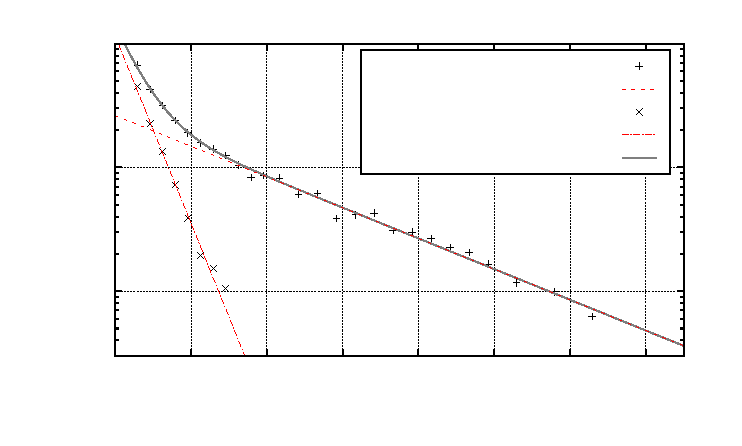
\includegraphics{dataanpassning}}%
    \gplfronttext
  \end{picture}%
\endgroup

\caption{Uppmätt och korrigerad aktivitet som funktion av tid med
  kurvanpassningar. De båda isotopernas aktivitet kan särskiljas genom
att i princip bara den ena isotopen finns kvar vid stora tider. Så en
exponentalanpassning kan göras till datan i den högra änden av
plotten. Därefter kan den kortlivade isotopens aktivitet extraheras
genom att subtrahera den första anpassingen från datan i den vänsta
änden. De anpassade havleringstiderna blev
$\Thalv{110}{Ag}=\unit[146]{s}$ och $\Thalv{108}{Ag}=\unit[24]{s}$.}
\label{fig:data}
\end{figure}


% \newpage
% \bibliographystyle{ieeetr}
% \bibliography{referenser}%kräver en fil som heter 'referenser.bib'          




\end{document}





%% På svenska ska citattecknet vara samma i både början och slut.
%% Använd två apostrofer (två enkelfjongar): ''.


%% Inkludera PDF-dokument
\includepdf[pages={1-}]{filnamn.pdf} %Filnamnet får INTE innehålla 'mellanslag'!

%% Figurer inkluderade som pdf-filer
\begin{figure}\centering
\centerline{ %centrerar även större bilder
\includegraphics[width=1\textwidth]{filnamn.pdf}
}
\caption{}
\label{fig:}
\end{figure}

%% Figurer inkluderade med xfigs "Combined PDF/LaTeX"
\begin{figure}\centering
\resizebox{.8\textwidth}{!}{\input{filnamn.pdf_t}}
\caption{}
\label{fig:}
\end{figure}

%% Figurer roterade 90 grader
\begin{sidewaysfigure}\centering
\centerline{ %centrerar även större bilder
\includegraphics[width=1\textwidth]{filnamn.pdf}
}
\caption{}
\label{fig:}
\end{sidewaysfigure}


%%Om man vill lägga till något i TOC
\stepcounter{section} %Till exempel en 'section'
\addcontentsline{toc}{section}{\Alph{section}\hspace{8 pt}Labblogg} 

